\chapter{分布式系统论文阅读}\label{chap:papers}
\addtocontents{los}{\protect\addvspace{10pt}}

\begin{intro}
整理阅读的分布式系统以及大数据处理方面的论文。
\end{intro}


\section{论文阅读要求}\label{sec:suggestions}

Cornell University CS6453%
\footnote{http://www.cs.cornell.edu/courses/cs6453/2017sp/index.html}%
给的阅读 paper 和准备 presentation 的建议

\textbf{Paper Reviews:} Please write constructive reviews. Here is a rough outline.
\begin{itemize}
	\item Summary of problem being solved (1-2 lines)
	\item Why is the problem interesting? Perhaps, its a new problem? Perhaps, its an old problem but with a new twist (e.g., new workloads, new environment, new hardware)? Perhaps, its just an old classical problem? (1-2 lines)
	\item What are the main insights in the proposed solution? What is the main technical contribution? How does the solution advance the state-of-the-art? (4-5 lines)
	\item Can you think of cases where the proposed solution may not work well? (4-5 lines)
	\item What are the next few problems that you would solve in this space? What do you think is the holy grail in this direction? (5-10 lines)
\end{itemize}

\textbf{Paper Presentations:} Please plan for 30 minutes. Here is a rough outline.
\begin{itemize}
	\item What is the problem being solved? (2-3 slides)
	\item Why is the problem interesting? Perhaps, its a new problem? Perhaps, its an old problem but with a new twist (e.g., new workloads, new environment, new hardware)? Perhaps, its just an old classical problem? (1-2 slides)
	\item What is the most related work and how is this paper different? (3-4 slides)
	\item What is the main technical contribution? What are the main insights used to build the proposed solution? How does the solution advance the state-of-the-art? (2-3 slides)
	\item Techniques used in the paper to solve the problem (4-5 slides)
	\item Can you think of cases where the proposed solution may not work well? (2-3 slides)
	\item What are the next few problems that you would solve in this space? What do you think is the holy grail in this direction? (4-5 slides)
\end{itemize}

所选择阅读并记录的论文参考自 Cornell CS6453 Spring2017%
\footnote{http://www.cs.cornell.edu/courses/cs6453/2017sp/schedule.html}%
和 MIT 6.824 Spring2018%
\footnote{https://pdos.csail.mit.edu/6.824/schedule.html}%

%
% 将各论文进行一个大的分类,在同一个 section 下
% 各论文讨论的东西作为 subsection 下
% 记录下阅读论文每个部分以及重读的时间,使用 【】 进行标记
%


\section{分布式存储}\label{sec:papers:storage}

\subsection{GFS}\label{paper:gfs}

\begin{itemize}
	\item [-] \textbf{The Google File System}
\end{itemize}

\begin{itemize}
	\item 【20180707】阅读了 Abstract \& Introduction 部分
	\item 
\end{itemize}

2003 年 Google 发表这篇论文,文中详细介绍了 Google 使用的分布式文件系统,其支持大规模分布式的数据密集型应用。那时候的计算机硬件特别昂贵且性能很差
(相较于现在,性价比应该是很低的),因此需要特别关注错误容忍(容错性,Fault Tolerance),集群中的任何一个节点可能在任何一个时间点宕机。

GFS 吸取了在其之前的众多分布式文件系统的特性,包括性能、可扩展性、可靠性、可用性(performance, scalability, reliability, and availability),
同时也根据 Google 具体的应用负载(application workloads)和应用环境(technological environment)进行了适配,重新审视了
传统分布式文件系统设计上的选择(choices),并提出了不同的系统设计考量。
\begin{enumerate}
	\item 集群中的组件故障(failures)是正常情况。在部署的分布式集群环境中,使用了成百上千台廉价的机器作为存储节点,这些组件宕掉是很正常的情况,
	因此所构建的系统需要满足(每一点都需要在之后补充上): %% TODO 
	\begin{itemize}
		\item constant monitoring
		\item error detection
		\item fault tolerance
		\item automatic recovery
	\end{itemize}
	\item 存储的文件非常大,比如 TB、PB 级别的数据
	\item 文件极少更新,更确切地说,文件作为某些计算的数据读入,并且不时有额外的数据追加到文件尾部
	\item 将文件系统的 API 与应用程序协同设计,以增加整个系统的灵活性
\end{enumerate}

\begin{newnote}[GFS 中为实现容错做了哪些手段?]
待补充 %% TODO Assign 20180707
\end{newnote}


\section{分布式计算}\label{sec:papers:computing}


\subsection{MapReduce}\label{paper:mapreduce}

\begin{itemize}
	\item [-] \textbf{MapReduce: Simplified Data Processing on Large Clusters}
\end{itemize}

\begin{itemize}
	\item %阅读 【20180707】
	\item 
\end{itemize}




\subsection{Spark}\label{paper:spark-and-rdd}

\begin{itemize}
	\item [-] \textbf{Spark: Cluster Computing with Working Sets}
	\item [-] \textbf{Resilient Distributed Datasets: A Fault-Tolerant Abstraction for In-Memory Cluster Computing}
\end{itemize}

\begin{itemize}
	\item %阅读 【20180707】 BSP
	\item 
\end{itemize}



\section{参数服务器}\label{sec:papers:ps}

\subsection{ASP}\label{paper:asp}

\begin{itemize}
	\item [-] \textbf{An Architecture for Parallel Topic Models}
\end{itemize}

\begin{itemize}
	\item %阅读 【20180707】
	\item 
\end{itemize}

2010 年的一篇文章,提出了参数服务器的概念,比较有开创性。

\subsection{SSP}\label{paper:ssp}

\begin{itemize}
	\item [-] \textbf{More Effective Distributed ML via a Stale Synchronous Parallel Parameter Server}
\end{itemize}

\begin{itemize}
	\item 【20180703】全文阅读,但跳过收敛性证明
	\item 【20180707】重读 \& 整理,同样跳过收敛性证明
\end{itemize}

这是分布式机器学习一个里程碑式的文章,提出了一个很 generic 的算法,提供了在某些合理假设下的收敛性证明(优化),并且在这个基础上
提出了一个合理的编程模型,最后给了一个系统实现。%
\footnote{https://zhuanlan.zhihu.com/p/29032307}%

在 Spark/Hadoop 中每个 worker 的新一次迭代都需要等待所有 workers 上一次迭代的结束,要用到上一次迭代的结果(BSP);
而对于 ASP,每一个 worker 执行调度器分配给自己的那部分任务,不用等待其他 workers 的执行。一个很直接的想法就是能否寻找一个折衷的
同步策略,即不是像 BSP 那样每次迭代都强制所有 workers 对上一次迭代进行同步,也不是像 ASP 那样各 workers 随意执行,而是每个 worker
都按照自己的节奏执行程序,但要求执行最快的那个 worker 与执行最慢的那个 worker 之间不能超过所指定的迭代数,例如 3 个迭代,如图
\ref{fig:paper-ssp} 所示。 

\begin{figure}[hbtp]
\centering
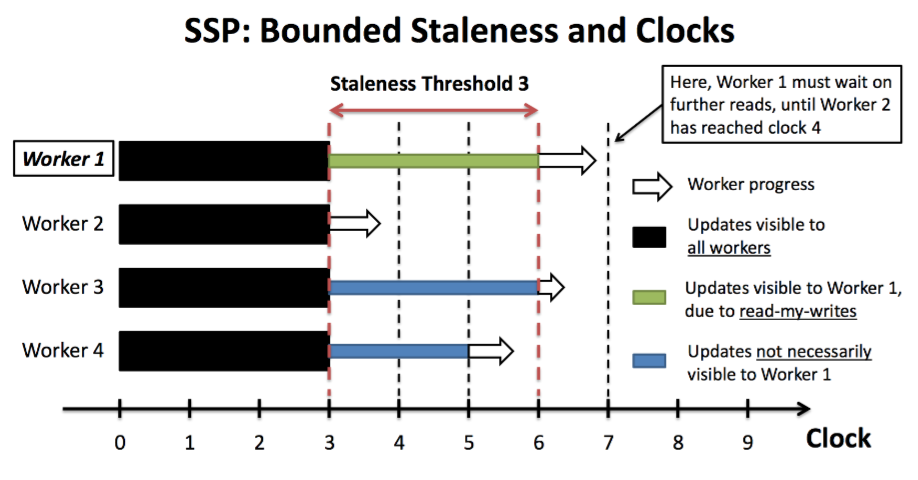
\includegraphics[width=0.65\textwidth]{paper-ssp}
\caption{SSP 模型示例}
\label{fig:paper-ssp}
\end{figure}

\begin{newnote}[摘录 SSP 论文中的描述]
We begin with an informal explanation of SSP: assume a collection of $P$ workers, each of which makes
additive updates to a shared parameter $x \gets x + \mu$ at regular intervals called \textit{clocks}.
Clocks are similar to iterations, and represent some unit of progress by an ML algorithm. Every worker
has its own integer-valued clock $c$, and workers only commit their updates at the end of each clock.
Updates may not be immediately visible to other workers trying to read $x$ --- in other words, workers
only see effects from a “stale” subset of updates. The idea is that, with staleness, workers can retrieve
updates from caches on the same machine (fast) instead of querying the parameter server over
the network (slow). Given a user-chosen staleness threshold $s \ge 0$, SSP enforces the following
bounded staleness conditions:

\begin{itemize}
	\item The slowest and fastest workers must be $\le s$ clocks apart --- otherwise, the fastest worker
	is forced to wait for the slowest worker to catch up.
	\item When a worker with clock $c$ commits an update $\mu$, that $\mu$ is timestamped with time $c$.
	\item When a worker with clock $c$ reads $x$, it will always see effects from all $\mu$ with timestamp
	$\le c - s - 1$. It may also see some $\mu$ with timestamp $> c - s - 1$ from other workers.
	\item Read-my-writes: A worker $p$ will always see the effects of its own updates up.
\end{itemize}
\end{newnote}


\subsection{Parameter Server}\label{paper:ps-osdi2014}

% http://chuansong.me/n/2161528 参数服务器——分布式机器学习的新杀器

\begin{itemize}
	\item [-] \textbf{Scaling Distributed Machine Learning with the Parameter Server}
	\item [-] \textbf{Communication Efficient Distributed Machine Learning with the Parameter Server}
\end{itemize}

\begin{itemize}
	\item 【20180625】阅读过好几遍了,打印纸质版、MarginNote 上,在笔记上手写了笔记
	\item 【20180707】重读 \& 整理
	\item 【20180708】整理,差论文 2.2 3.4 的理解与整理,可能需要看过 ps-lite 代码之后才能理解的更清晰
\end{itemize}

沐帅在 OSDI 2014 上发表这篇工作,引出第三代参数服务器框架,在 worker 节点上分布式存放数据和工作负载,server 节点上保存着
全局共享的参数,各节点之间异步通信,支持灵活的一致性模型,可扩展并且容错性很好(continuous fault tolerance 是什么意思)。

当处理大规模的机器学习(深度学习)模型时,会面临这样一个问题:多台机器节点之间需要共享一些状态信息,包括参数、集群信息,用户 profiles
以及其他一些需要在各节点之间进行交流的信息。另外,单机已经解决不了目前快速增长的数据和参数了,在实际的系统中训练的数据量已经达到 TB、PB
级别,训练过程中可能会产生 $10^9 \sim 10^{12}$ 的参数量(这两个数据是在 2014 年年初时候的数据,现在需要更新了)。%% TODO
模型参数被所有的 worker 节点所共享并且会被频繁访问到,这就会带来很多问题和挑战:
\begin{enumerate}
	\item 访问这些巨量的参数,需要大量的网络带宽支持
	\item 很多机器学习算法是连续型的(顺序的),只有上一次迭代完成(各个 worker 上都完成)之后,才能进行下一次迭代,这导致如果
	各机器之间的性能差距太大(木桶效应),就会造成性能的极大损失(因为系统整体的性能由性能最差的那台机器所决定)
	\item 在分布式系统中容错能力是非常重要的,在真实环境的部署下,算法最终是在云上(云计算)运行的(这种环境下,机器是不可靠的,
	并且所提交的 job 可能会被其他任务抢占)
\end{enumerate}

沐帅将参数服务器的发展分为三个阶段:
\begin{itemize}
	\item [第一代] 缺少灵活性和性能 --- 仅使用 memcached 分布式 (key, value) 存储,来作为同步机制。YahooLDA
	通过改进这一机制,增加了一个专门的服务器,提供用户能够自定义的更新操作(set/get/update)
	\item [第二代] Petuum 使用 bounded delay 模型来改进 YahooLDA,但是却限制了 worker 的线程模型
	\item [第三代] 即在这篇 paper 中提出来,能够解决这些局限性
\end{itemize}

参数服务器与通用的分布式系统有什么区别呢?通用的分布式系统通常是每次迭代都强制同步,在十几个节点上它们的性能可以表现的很好,但是
在大规模集群中,这样的每次迭代强制同步的机制(BSP)会因为木桶效应变得很慢。Mahout 基于 Hadoop,MLI 基于 Spark,它们
(MLI 和 Spark)采用的都是 Iterative MapReduce 架构,能够保持迭代之间的状态,并且执行策略也更加优化了,但是由于这两种方法
均采用了同步迭代的通信方式,使得它们很容易因为个别机器的低性能导致全局性能的降低。为了解决这个问题,GraphLab 采用图形抽象的方式
进行异步通信,但是它缺少以 MapReduce 为基础架构的弹性扩展性,并且它使用粗粒度的 snapshots 来进行恢复,这两点都会阻碍到可扩展性。

参数服务器正是吸取了两者的优点,1)MLI 和 Spark 保持各个迭代之间的状态信息,2)GraphLab 异步通信,并且解决了 GraphLab 在
可扩展性方面的劣势。

\noindent\textbf{Distributed Subgradient Descent} 论文的 2.2 节 %% TODO 待整理

\noindent\textbf{架构}

一个参数服务器的实例可以同时运行多个算法。参数服务器的节点以 group 进行分组,包含一个 server group 和多个 worker group,
如图 \ref{fig:paper-ps-architecture} 所示。

\begin{figure}[hbtp]
\centering
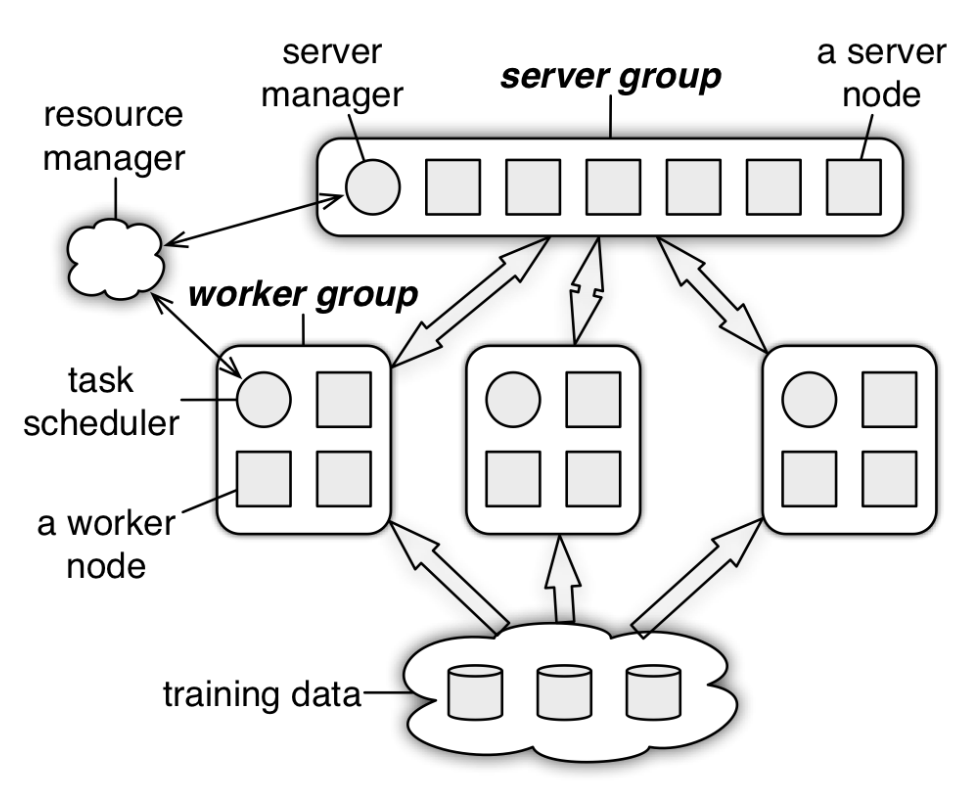
\includegraphics[width=0.65\textwidth]{paper-ps-architecture}
\caption{参数服务器的架构}
\label{fig:paper-ps-architecture}
\end{figure}

在 server group 中的每一个 server 节点保存着部分全局共享的参数,每个 server 节点之间会进行通信,以进行备份或者迁移节点上的参数,
这是为了整个系统的容错性和可扩展性考虑。在 server group 中有一个节点的角色是 server manager,保存各 server 节点的元数据信息
(包括节点是否存活,分配在其上的共享参数的范围),需要考虑如何保持一致性。

每一个 worker group 上都运行着一个应用。每一个 worker 节点上都本地保存着部分的训练数据,用来计算一个本地的梯度值。worker 节点
将计算得到的梯度值 push 给 server 节点,或者从 server 节点上 pull 下已更新的参数;各 worker 节点之间不进行通信。每一个 worker
group 中同样有一个 task scheduler 节点,负责分配任务给 group 中的所有 worker 节点,并监测各 worker 的执行进度,在新的 worker
节点添加进该 group 或有 worker 节点被移除时,scheduler 节点负责重新调度未完成的任务。

参数服务器支持独立的参数命名空间(namespace)。

沐帅提出的第三代参数服务器包含以下几个要点:
\begin{itemize}
	\item 所有共享参数的形式都是 (key, value) vectors --- 假设 keys 是有序的,不存在的 key 对应的 value 值为 0
	\item 基于 range 的 push/pull 操作,这样 worker 节点每次与 server 节点进行通信时可以选择性的仅传递少量需要更新的参数,
	更可控也更灵活
	\item server 节点用于聚集各 worker 节点发送过来的各子梯度值,同时,server 节点也支持执行用户指定的操作。支持这样的操作是很有
	好处的,因为 server 节点通常保存有更完整并且更 up-to-date 的共享参数信息
	\item 异步操作,回调的实现 %% TODO
	\item 各 worker 节点异步的执行任务,各节点之间可能会出现数据不一致,从而使得算法的收敛过程变慢。然而,有一些算法对数据的一致性
	要求没有那么严格,即有一些算法在数据出现不一致时,也能够在最终收敛并得到准确的结果。

	对一致性协议的考量,需要在系统性能跟算法收敛速率之间做一个 tradeoff,同时考虑:
	\begin{enumerate}
		\item 算法对于参数非一致性的敏感程度
		\item 训练数据的特征之间的关联度
		\item 硬件设备的能力
	\end{enumerate}

	考虑到用户使用的时候会有不同的情况,参数服务器为用户提供了多种任务依赖方式,1)Sequential,2)Eventual,3)Bounded delay
	\item 用户可自定义的过滤器。对于机器学习优化问题来说,比如梯度下降,并不是每次计算的梯度对于最终优化都是有价值的,用户可以通过
	自定义的规则过滤一些不必要的通信,再进一步压缩带宽耗费:
	\begin{enumerate}
		\item 发送很小的梯度值是低效的 --- 因此可以自定义设置,只在梯度值很大的时候发送
		\item 更新接近最优情况的值是低效的 --- 因此只在非最优情况下发送,可通过 KKT 条件来判断
	\end{enumerate}
\end{itemize}

%% 待补充什么呢?


\subsection{GeePS}\label{paper:geeps}

\begin{itemize}
	\item [-] \textbf{GeePS: Scalable deep learning on distributed GPUs with a GPU-specialized parameter server}
\end{itemize}

\begin{itemize}
	\item %【20180707】阅读
	\item 
\end{itemize}



% \section{}\label{sec:papers:}

% \subsection{}\label{}

% \subsection{}\label{}

% \subsection{}\label{}


\endinput
